\documentclass[../../main.tex]{subfiles}
\begin{document}

{\bf [解答]}

% TODO: 正十二角形と外接する半径1の円の図
\begin{figure}[htb]
  \centering
  \begin{tikzpicture}[scale=2.0, >=stealth, every node/.style={font=\small}]

    \coordinate (O) at (0, 0);

    % --- 1. 外接円 (半径 1) ---
    \draw[thick, gray!60] (O) circle (1.0);
    \node[gray!80!black, font=\scriptsize, above right] at (45:1.0) {円（半径 $1$）};

    % --- 2. 正十二角形（内接） ---
    \draw[very thick, blue!85!black]
    (0:1.0) \foreach \ang in {30, 60, ..., 360} { -- (\ang:1.0) };

    % --- 3. 中心からの分割動径線（点線） ---
    \foreach \ang in {0, 30, ..., 330} {
      \draw[dashed, gray!45] (O) -- (\ang:1.0);
      \fill[blue!90!black] (\ang:1.0) circle (0.8pt);
    }

    % 中心点
    \fill[black] (O) circle (1.0pt) node[below left=1pt] {$O$};

    % 半径 1 と 1 辺 l のラベル
    \node[teal!90!black, font=\scriptsize, above] at (15:0.5) {$1$};
    \node[teal!90!black, font=\scriptsize, below] at (-15:0.5) {$1$};
    \node[red!90!black, font=\scriptsize\bfseries, right] at (15:1.0) {$l$};

  \end{tikzpicture}
  \caption{半径 $1$ の円に内接する正十二角形}
  \label{fig:dodecagon_inscribed_circle}
\end{figure}

上図のように半径$1$の円に内接する正十二角形を考える．
この1辺の長さを $l$ として，これは円周の長さより短いから
\begin{align}
  12l < 2\pi \iff 6l < \pi \label{eq:1}
\end{align}
である．

% TODO: 正十二角形の隣り合う頂点と中心からなる三角形の図
\begin{figure}[htb]
  \centering
  \begin{tikzpicture}[scale=3.2, >=stealth, every node/.style={font=\small}]

    % --- 1. 座標定義 ---
    % 中心角 30° の二等辺三角形 (2辺が 1, 底辺が l)
    \coordinate (O) at (0, 0);
    \coordinate (A) at (1.0, 0);
    \coordinate (B) at (30:1.0);

    % --- 2. 三角形の描画 ---
    \fill[blue!10, opacity=0.7] (O) -- (A) -- (B) -- cycle;
    \draw[very thick, blue!85!black] (O) -- (A) -- (B) -- cycle;

    % --- 3. 中心角 pi/6 の円弧 ---
    \draw[->, thick, purple!85!black] (0.35, 0) arc (0:30:0.35);
    \node[purple!90!black, font=\footnotesize\bfseries] at (15:0.48) {$\frac{\pi}{6}$};

    % --- 4. 辺の長さラベル ---
    \node[below=2pt, font=\scriptsize] at ($ (O)!0.5!(A) $) {$1$};
    \node[above left=1pt, font=\scriptsize] at ($ (O)!0.5!(B) $) {$1$};
    \node[right=2pt, font=\footnotesize\bfseries, red!85!black] at ($ (A)!0.5!(B) $) {$l$};

    % 頂点プロット
    \fill[black] (O) circle (0.8pt) node[left=2pt] {$O$};
    \fill[black] (A) circle (0.8pt);
    \fill[black] (B) circle (0.8pt);

  \end{tikzpicture}
  \caption{正十二角形の中心と隣り合う 2 頂点がつくる三角形}
  \label{fig:dodecagon_subtriangle}
\end{figure}

一方で，正十二角形の隣り合う頂点と中心からなる三角形に余弦定理を用いると
\begin{align}
  l^2 = 1+1 - 2\cdot 1\cdot 1\cdot \dfrac{\sqrt{3}}{2} = 2-\sqrt{3} \label{eq:2}
\end{align}
である．従って\cref{eq:1}に代入して
\begin{align}
  \pi^2 > 36(2-\sqrt{3}) \label{eq:3}
\end{align}
である．ここで$(3.05)^2$と$36(2-\sqrt{3})$の大小を比べよう．
\begin{align}
  (3.05)^2 &< 36(2-\sqrt{3}) \\
  \iff \sqrt{3} &< 2 - \dfrac{(3.05)^2}{36} \\
  \iff 3 &< 4 - \dfrac{(3.05)^2}{9} + \dfrac{(3.05)^4}{36^2} \quad \text{(両辺2乗)} \\
  \iff 0 &< 1 - \dfrac{(3.05)^2}{9} + \dfrac{(3.05)^4}{36^2}
\end{align}
だが，この右辺は，
\begin{align}
  (\text{右辺})
  = 1 - \dfrac{9.3025}{9}\left(1-\dfrac{9.3025}{144}\right)
  > 1 - \dfrac{9.3025}{9}\dfrac{134.7}{144}
  > \dfrac{42}{1296} > 0
\end{align}
となるから，$(3.05)^2 < 36(2-\sqrt{3})$ である．よって\cref{eq:3}より
\begin{align}
  (3.05)^2 < \pi^2 \quad \therefore 3.05 < \pi \quad (\because \pi > 0)
\end{align}
である．

{\bf [別解1]}

% TODO: x^2+y^2=25の四分円，(0,5),(3,4),(4,3),(5.0)を結んだ折れ線の図
\begin{figure}[htb]
  \centering
  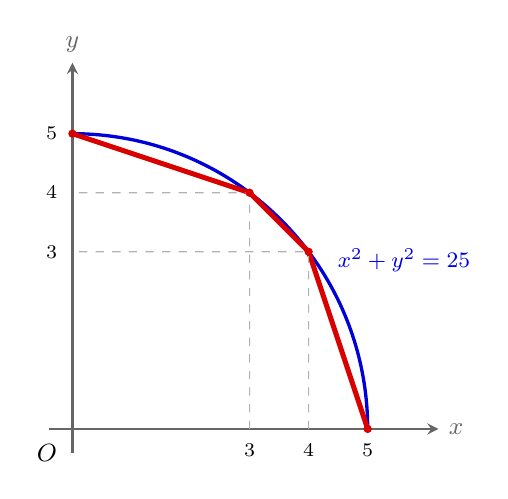
\begin{tikzpicture}[scale=0.75, >=stealth, every node/.style={font=\small}]

    % --- 1. 座標定義 ---
    \coordinate (O)  at (0, 0);
    \coordinate (P0) at (0, 5);
    \coordinate (P1) at (3, 4);
    \coordinate (P2) at (4, 3);
    \coordinate (P3) at (5, 0);

    % --- 2. 座標軸 ---
    \draw[->, thick, gray!80!black] (-0.4, 0) -- (6.2, 0) node[right] {$x$};
    \draw[->, thick, gray!80!black] (0, -0.4) -- (0, 6.2) node[above] {$y$};
    \node[below left=2pt] at (O) {$O$};

    % --- 3. 四分円 x^2 + y^2 = 25 (半径 5) ---
    \draw[very thick, blue!85!black] (5, 0) arc (0:90:5);
    \node[blue!90!black, font=\footnotesize\bfseries, above right] at (30:5) {$x^2+y^2=25$};

    % --- 4. 内接折れ線 (0,5)-(3,4)-(4,3)-(5,0) ---
    \draw[line width=1.8pt, red!85!black] (P0) -- (P1) -- (P2) -- (P3);

    % --- 5. 投影破線と目盛り ---
    \draw[dashed, gray!60] (3, 0) -- (P1) -- (0, 4);
    \draw[dashed, gray!60] (4, 0) -- (P2) -- (0, 3);

    \node[below=2pt, font=\scriptsize] at (3, 0) {$3$};
    \node[below=2pt, font=\scriptsize] at (4, 0) {$4$};
    \node[below=2pt, font=\scriptsize] at (5, 0) {$5$};

    \node[left=2pt, font=\scriptsize] at (0, 3) {$3$};
    \node[left=2pt, font=\scriptsize] at (0, 4) {$4$};
    \node[left=2pt, font=\scriptsize] at (0, 5) {$5$};

    % 格子点のプロット
    \fill[red!85!black] (P0) circle (2.0pt);
    \fill[red!85!black] (P1) circle (2.0pt);
    \fill[red!85!black] (P2) circle (2.0pt);
    \fill[red!85!black] (P3) circle (2.0pt);

  \end{tikzpicture}
  \caption{四分円 $x^2+y^2=25$ と 4 つの格子点を結ぶ内接折れ線}
  \label{fig:quarter_circle_chords}
\end{figure}

上図で折れ線の長さより四分円の円弧の方が長いから
\begin{align}
  4(2\sqrt{10} + \sqrt{2}) < 10\pi
\end{align}
左辺は $30.955\dots$ だから，$3.05 < \pi$ は示された．

{\bf [別解2]}

% TODO: 面積評価の図
\begin{figure}[htb]
  \centering
  \begin{tikzpicture}[x=5.5cm, y=3.2cm, >=stealth, every node/.style={font=\small}]

    % --- 1. 定数・厳密パラメータ ---
    % x_0 = 0, y_0 = 1
    % x_1 = 1/(2*sqrt(3)) = sqrt(3)/6 ≈ 0.2887
    %   y_1 = 1 / (1 + 1/12) = 12/13 ≈ 0.9231
    % x_2 = 1/sqrt(3) = sqrt(3)/3 ≈ 0.5774
    %   y_2 = 1 / (1 + 1/3) = 3/4 = 0.75
    \def\xMid{0.288675}
    \def\xEnd{0.577350}
    \def\yMid{0.923077} % 12/13
    \def\yEnd{0.750000} % 3/4

    \coordinate (O)  at (0, 0);
    \coordinate (P0) at (0, 1.0);
    \coordinate (P1) at (\xMid, \yMid);
    \coordinate (P2) at (\xEnd, \yEnd);

    % --- 2. 2つの内接台形の塗りつぶし ---
    \fill[pattern=north east lines, pattern color=blue!65, opacity=0.7]
    (0, 0) -- (P0) -- (P1) -- (P2) -- (\xEnd, 0) -- cycle;

    % --- 3. 座標軸 ---
    \draw[->, thick, gray!80!black] (-0.1, 0) -- (0.8, 0) node[right] {$x$};
    \draw[->, thick, gray!80!black] (0, -0.1) -- (0, 1.25) node[above] {$y$};
    \node[below left=2pt] at (O) {$O$};

    % --- 4. 曲線 y = 1 / (1 + x^2) ---
    \draw[very thick, blue!85!black, domain=0:0.7, samples=60]
    plot (\x, {1.0 / (1.0 + \x*\x)});
    \node[blue!90!black, font=\footnotesize\bfseries, above right] at (0.35, 0.95)
    {$y = \frac{1}{1+x^2}$};

    % --- 5. 台形の上底（折れ線 P0 - P1 - P2）---
    \draw[line width=1.6pt, red!85!black] (P0) -- (P1) -- (P2);

    % --- 6. 縦の分割線と投影破線 ---
    \draw[thick, gray!75!black] (\xMid, 0) -- (P1);
    \draw[thick, gray!75!black] (\xEnd, 0) -- (P2);

    \draw[dashed, gray!50] (0, \yMid) -- (P1);
    \draw[dashed, gray!50] (0, \yEnd) -- (P2);

    % --- 7. 目盛りとラベル ---
    \node[below=2pt, font=\scriptsize] at (\xMid, 0) {$\frac{\sqrt{3}}{6}$};
    \node[below=2pt, font=\scriptsize] at (\xEnd, 0) {$\frac{\sqrt{3}}{3}$};

    \node[left=2pt, font=\scriptsize] at (0, 1.0) {$1$};
    \node[left=2pt, font=\scriptsize] at (0, \yMid) {$\frac{12}{13}$};
    \node[left=2pt, font=\scriptsize] at (0, \yEnd) {$\frac{3}{4}$};

    % 点のプロット
    \fill[black] (P0) circle (0.8pt);
    \fill[red!85!black] (P1) circle (1.0pt);
    \fill[red!85!black] (P2) circle (1.0pt);

  \end{tikzpicture}
  \caption{上に凸な関数 $y = \dfrac{1}{1+x^2}$ と 2 つの台形による下からの面積評価}
  \label{fig:trapezoid_integration_pi_bound}
\end{figure}

$[0,\dfrac{\sqrt{3}}{3}]$で上に凸な関数$y=\dfrac{1}{1+x^2}$の積分をしたから台形で評価すると，
\begin{align}
  \int_0^{1/\sqrt{3}} \dfrac{1}{1+x^2} dx
  &> \dfrac{1}{2} \cdot \dfrac{\sqrt{3}}{6} \dfrac{25}{13} + \dfrac{1}{2} \cdot \dfrac{\sqrt{3}}{6} \left( \dfrac{12}{13} + \dfrac{3}{4} \right) \\
  & \dfrac{\pi}{6} > \dfrac{\sqrt{3}}{12} \left( \dfrac{25}{13} + \dfrac{12}{13} + \dfrac{3}{4} \right) \\
  & \pi > \dfrac{\sqrt{3}}{2} \left( \dfrac{37}{13} + \dfrac{3}{4} \right)
\end{align}
である．右辺を計算すると$\pi > 3.114\cdots$ となり題意は示された．

{\bf [別解3]}

$\cos x \ge 1 - \dfrac{1}{2}x^2$ に $x = \pi/6$ を代入して
\begin{align}
  \dfrac{\sqrt{3}}{2} \ge 1 - \dfrac{\pi^2}{72} \quad \therefore \pi \ge \sqrt{72-36\sqrt{3}} = 3.105\dots
\end{align}
となり示された．

\end{document}
